\section{Adapted PPO Algorithm} \label{appendix:ppo}
As defined in \cref{sec:algorithmic_details} the loss function for the global value function is 
\[ L_{\mathcal{V}}(\boldsymbol O^n, \boldsymbol{G}^n, \phi) =  ||\mathcal V^{FCN}_{\phi}(\boldsymbol O^n)- \boldsymbol{G}^n||_2^2. \]
We note that this notation contains the parameters $\phi$, which parameterize the underlying neural network.

The objective for the global policy is defined as
\[L_{\Pi}(\boldsymbol O^n, \boldsymbol A^n, \theta_k, \theta, \beta) := \frac{1}{\tilde N_x\cdot \tilde N_y} \sum_{i,j=1}^{\tilde N_x, \tilde N_y} L_{\pi_{ij}}({O}^n_{ij}, {A}^n_{ij}, \theta_k, \theta) - \beta H(\pi_{ij,\theta}),\]
where  $H(\pi_{ij,\theta})$ is the entropy of the local policy and $L_{\pi_{ij}}$ is the standard single-agent PPO-Clip objective
\[ \label{eq:ppo_objective}
L_{\pi_{ij}}(o, a, \theta_k, \theta) = \min \left( \frac{\pi_{ij,\theta}(a|o)}{\pi_{ij,\theta_k}(a|o)} Adv^{\pi_{ij,\theta_k}}(o, a), \text{clip} \left( \frac{\pi_{ij,\theta}(a|o)}{\pi_{ij,\theta_k}(a|o)}, 1 - \epsilon, 1 + \epsilon \right) Adv^{\pi_{ij,\theta_k}}(o, a) \right).
\]
The advantage estimates \( {Adv}^{\pi_{ij,\theta_k}} \) are computed with generalized advantage estimation (GAE) \cite{generalized_advantage_estimation} using the output of the global value network \( \mathcal{V}^{FCN}_{\phi} \).\\

The resulting adapted PPO algorithm is presented in \cref{algo:ppo}. Major differences compared to the original PPO algorithm are vectorized versions of the value network loss and PPO-Clip objective, as well as a summation over all the discretization points of the domain before performing an update step.  

\begin{algorithm}[tb]
   \caption{Adapted PPO Algorithm}
    \label{algo:ppo}
\begin{algorithmic}
   \STATE {\bfseries Input:} Initial policy parameters \( \theta_1 \), initial value function parameters \( \phi_1 \), \\
 clip ratio \( \epsilon\), discount factor \(\gamma\), entropy regularization weight \(\beta\)
   \FOR{\( k = 1, 2, \ldots \)}
   \STATE Collect set of trajectories \( D_k  \) with the  global policy \( \Pi^{FCN}_{\theta_k} \) in the environment
   \STATE \textit{\# Update global policy}
   \STATE Update $\theta$ by performing a SGD step on \( \theta_{k+1} = \arg \max_\theta \frac{1}{\|D_k\|}\sum_{\boldsymbol{O}^n, \boldsymbol G^n \in D_k} L_{\Pi}(\boldsymbol O^n, \boldsymbol A^n, \theta_k, \theta, \beta) \)
   \STATE \textit{\# Update global value network}
    \STATE Compute returns for each transition using \( \boldsymbol{G}^n=\sum_{i=n}^N \gamma^{i-t} \boldsymbol{R}^i \) where $N$ is the length of the respective trajectory
    \STATE Update $\phi$ by performing a SGD step on \( \phi_{k+1} = \arg \min_\phi \frac{1}{\|D_k\|}\sum_{\boldsymbol{O}^n, \boldsymbol G^n \in D_k} L_{\mathcal V}(\boldsymbol{O}^n, \boldsymbol{G}^n, \phi) \)
   \ENDFOR
\end{algorithmic}
\end{algorithm}

\newpage
\section{Additional Results}
\subsection{Advection Equation}
\begin{figure}[ht]
\vskip 0.2in
\begin{center}
\centerline{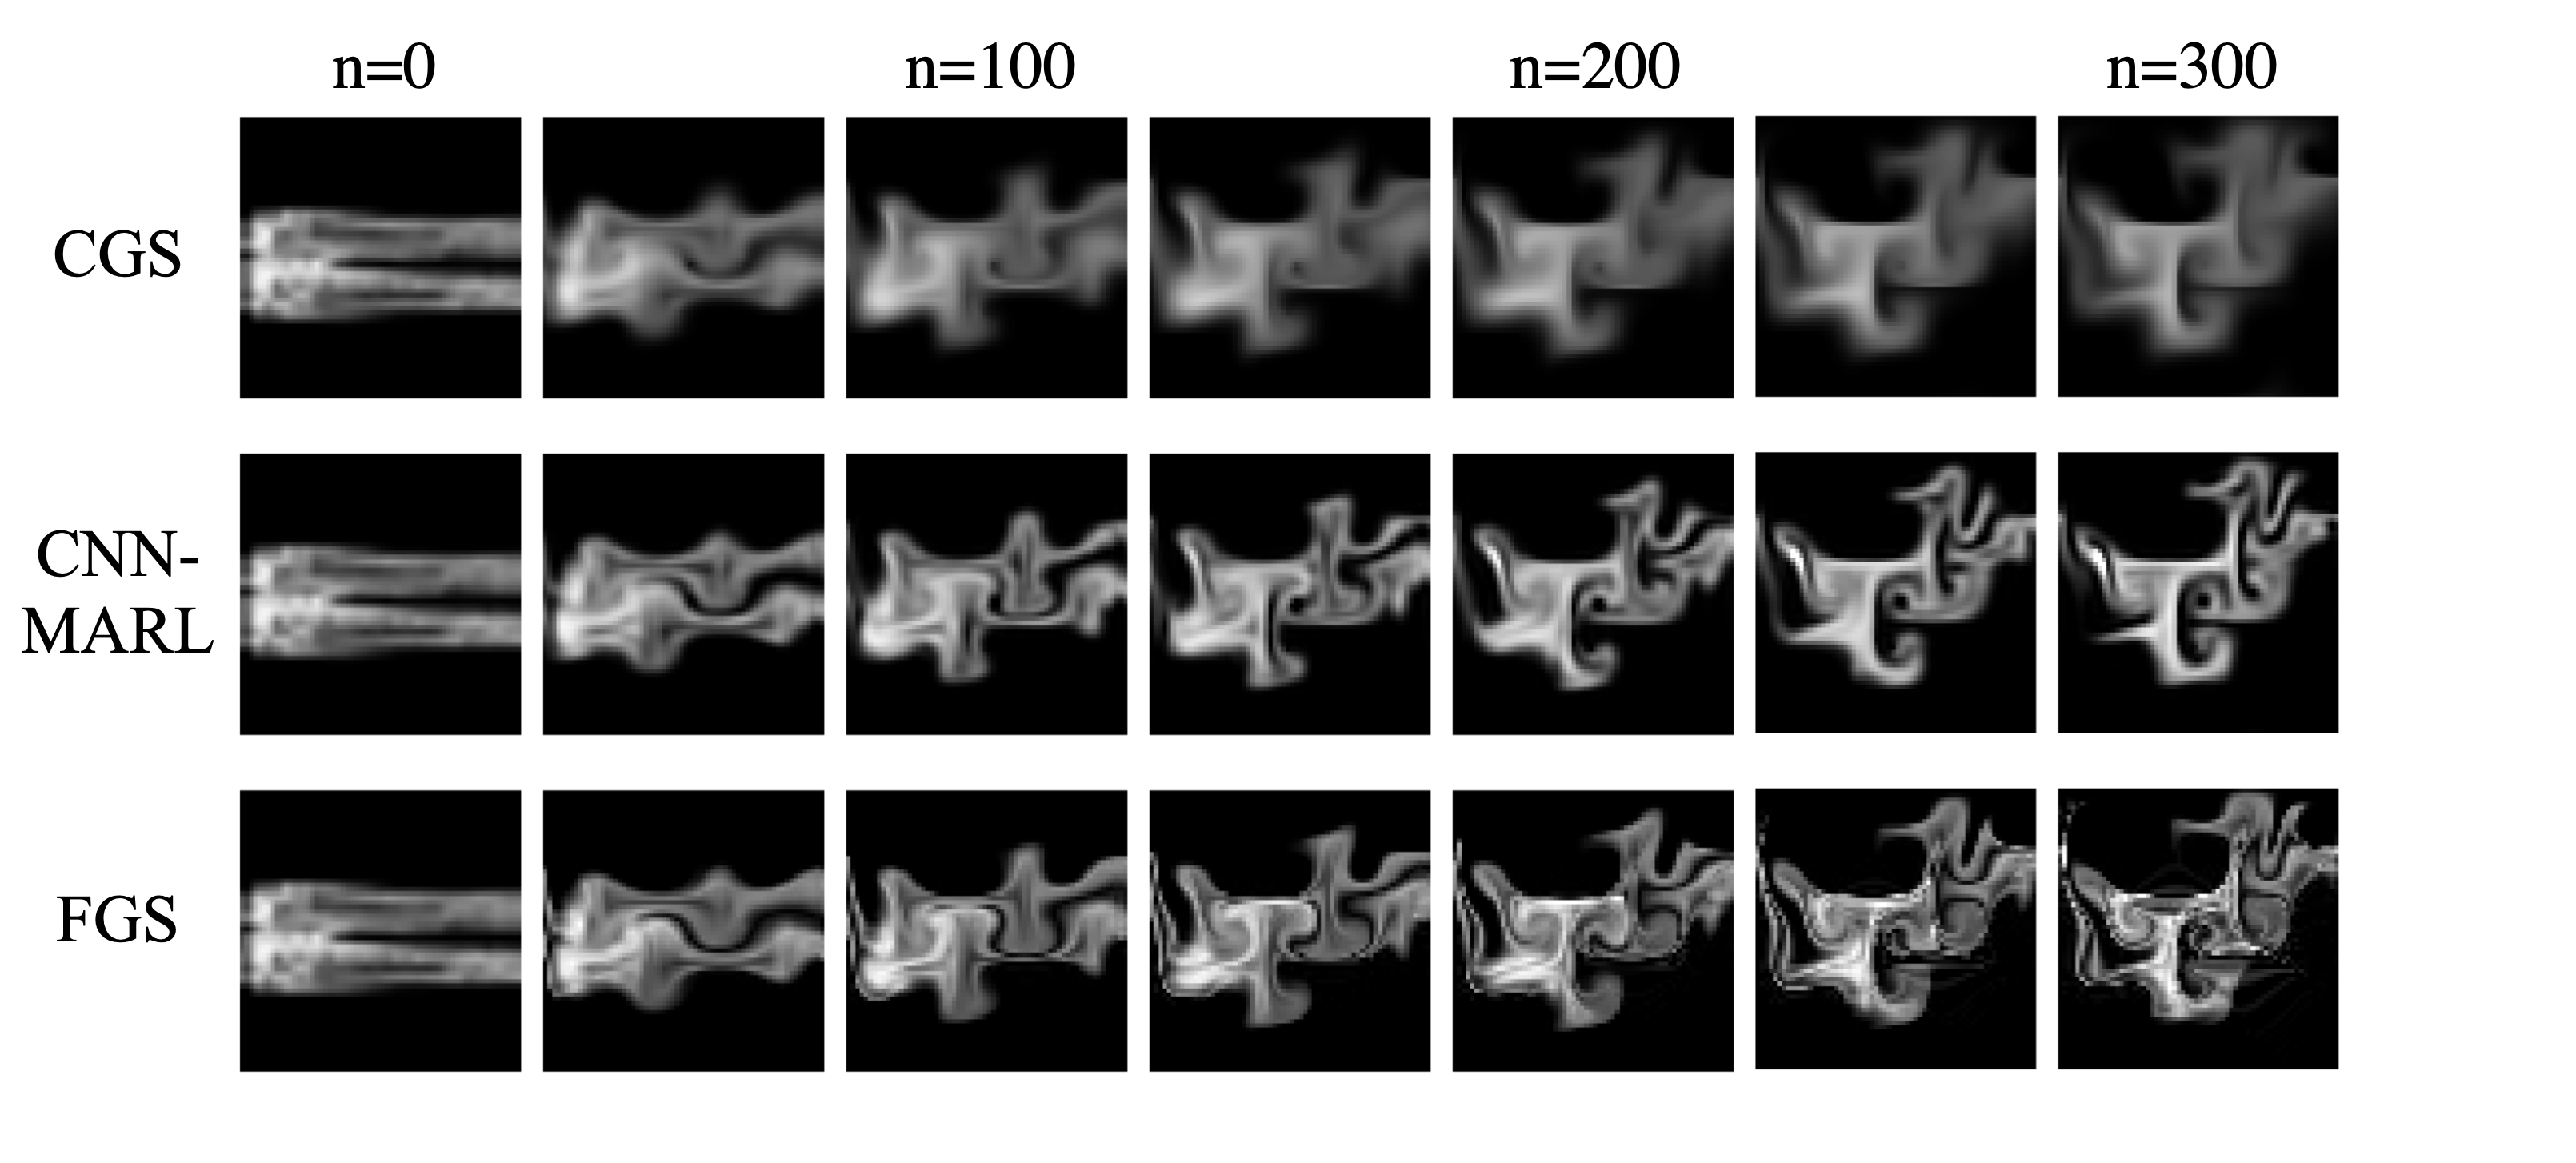
\includegraphics[width=0.75\columnwidth]{illustrations/advection/fashion_train_illustration.png}}
\caption{$\boldsymbol \psi^0$ is sampled from the MNIST test set. The velocity field is sampled from $\mathcal D^{Vortex}_{Test}$ (See \cref{sec:train_vortices}). Here, the IC of the concentration comes from a different distribution than the one used for training.}
\end{center}
\vskip -0.2in
\end{figure}

\begin{figure}[ht]
\vskip 0.2in
\begin{center}
\centerline{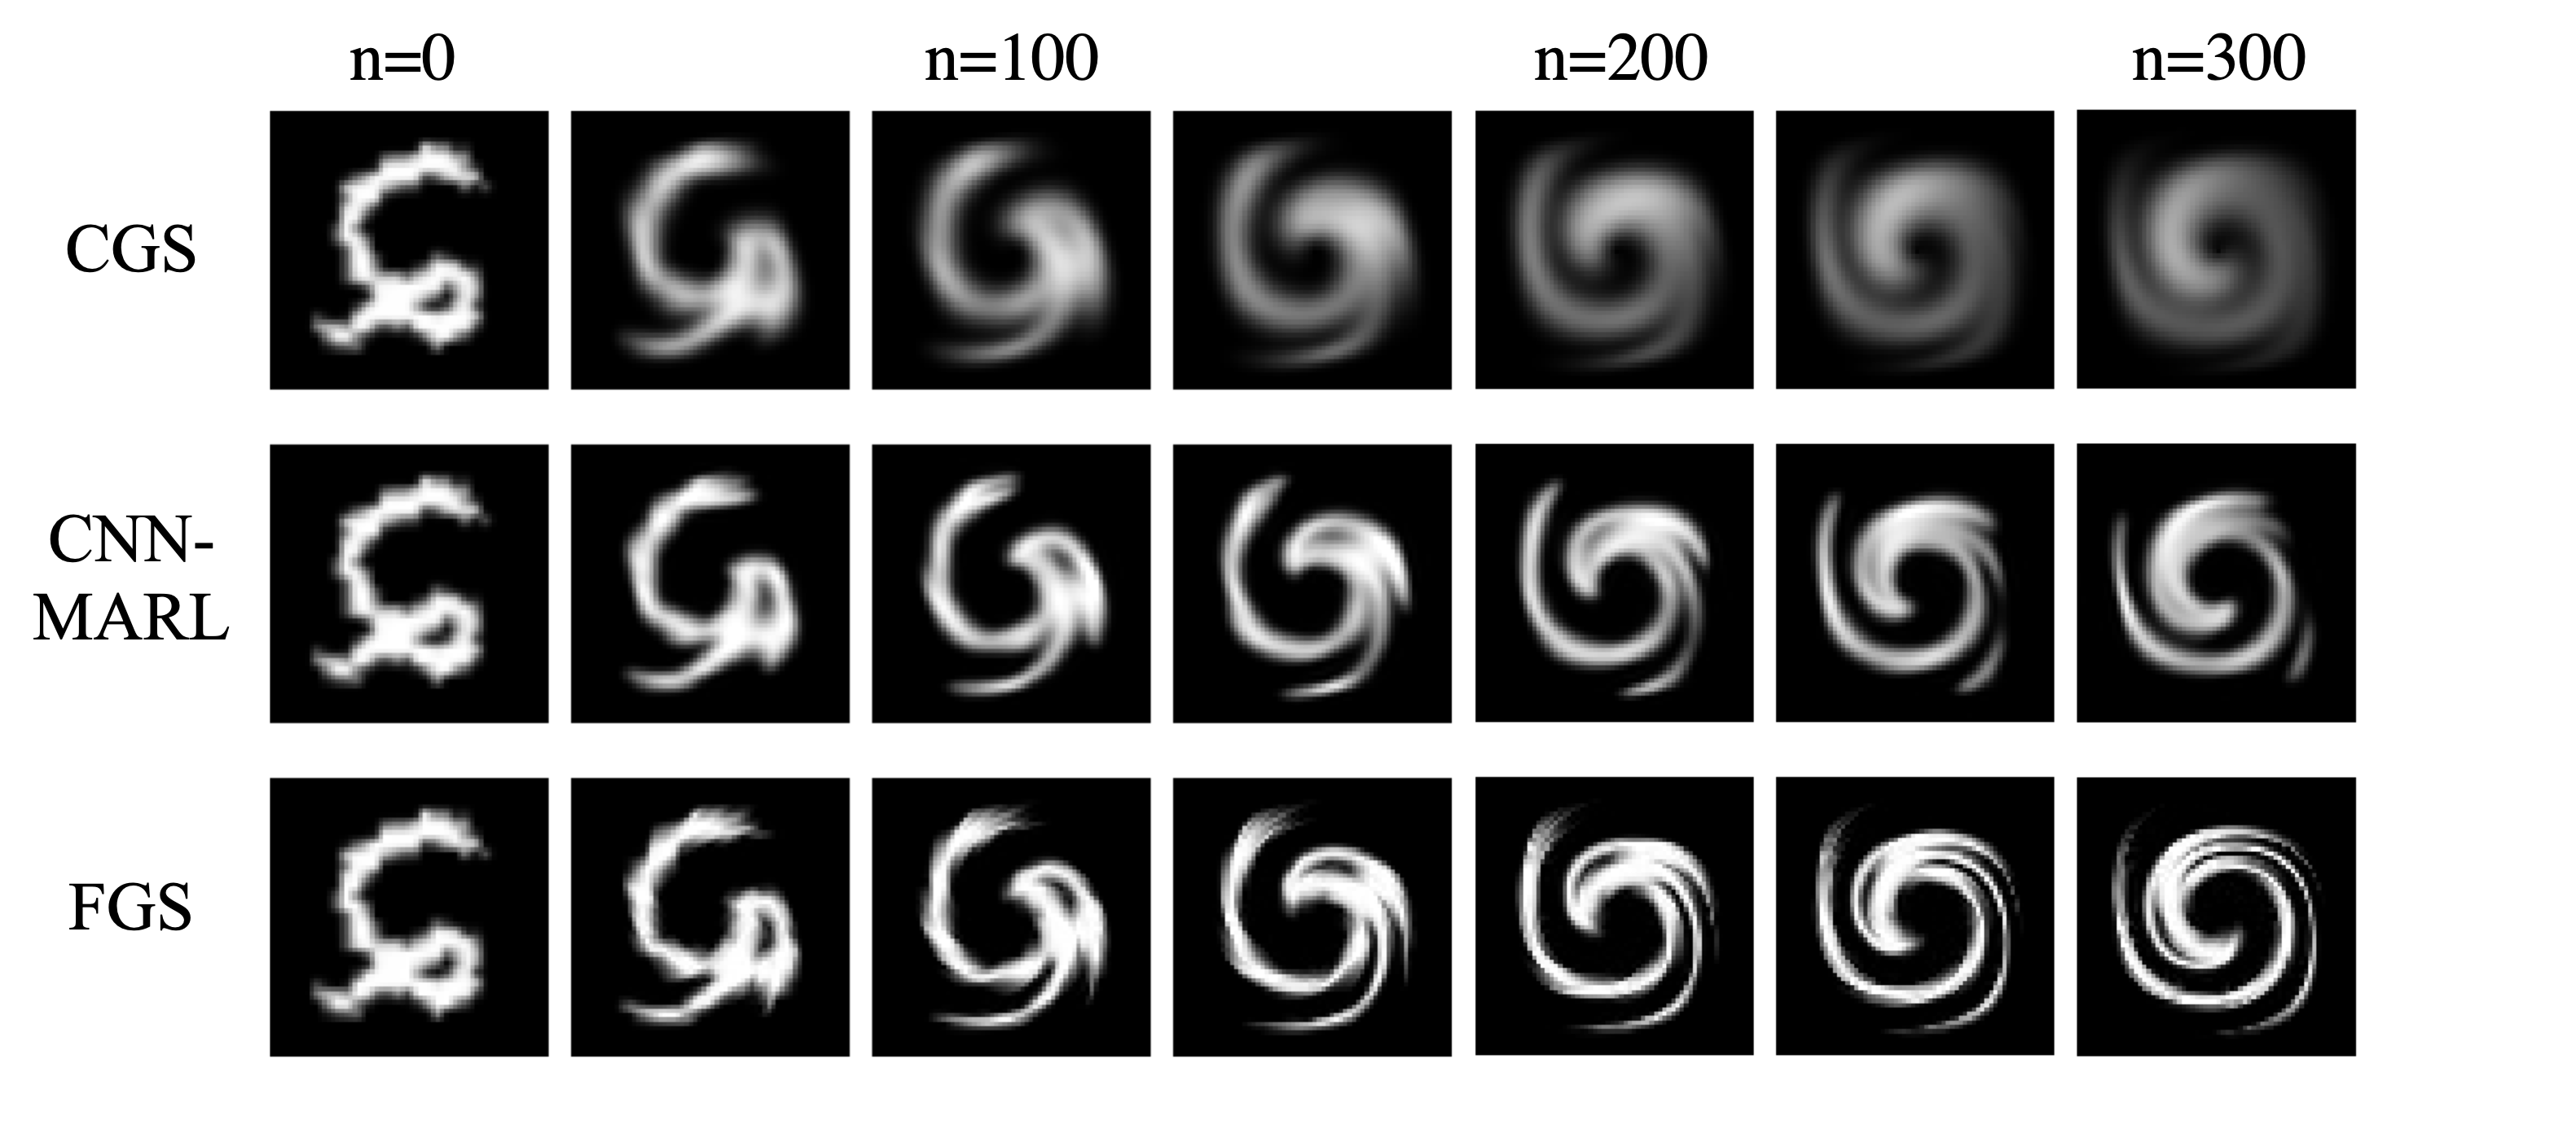
\includegraphics[width=0.75\columnwidth]{illustrations/advection/mnist_vortex_illustration.png}}
\caption{$\boldsymbol \psi^0$ is a sample from the F-MNIST test set. The velocity field is sampled from $\mathcal D^{Vortex}_{Train}$ (See \cref{sec:test_vortices}). Note that the velocity field comes from a different distribution than the one used for training.}
\end{center}
\vskip -0.2in
\end{figure}

\newpage
\subsection{Burgers' Equation}
\label{sec:adres}
\begin{figure}[ht]
\vskip 0.2in
\begin{center}
\centerline{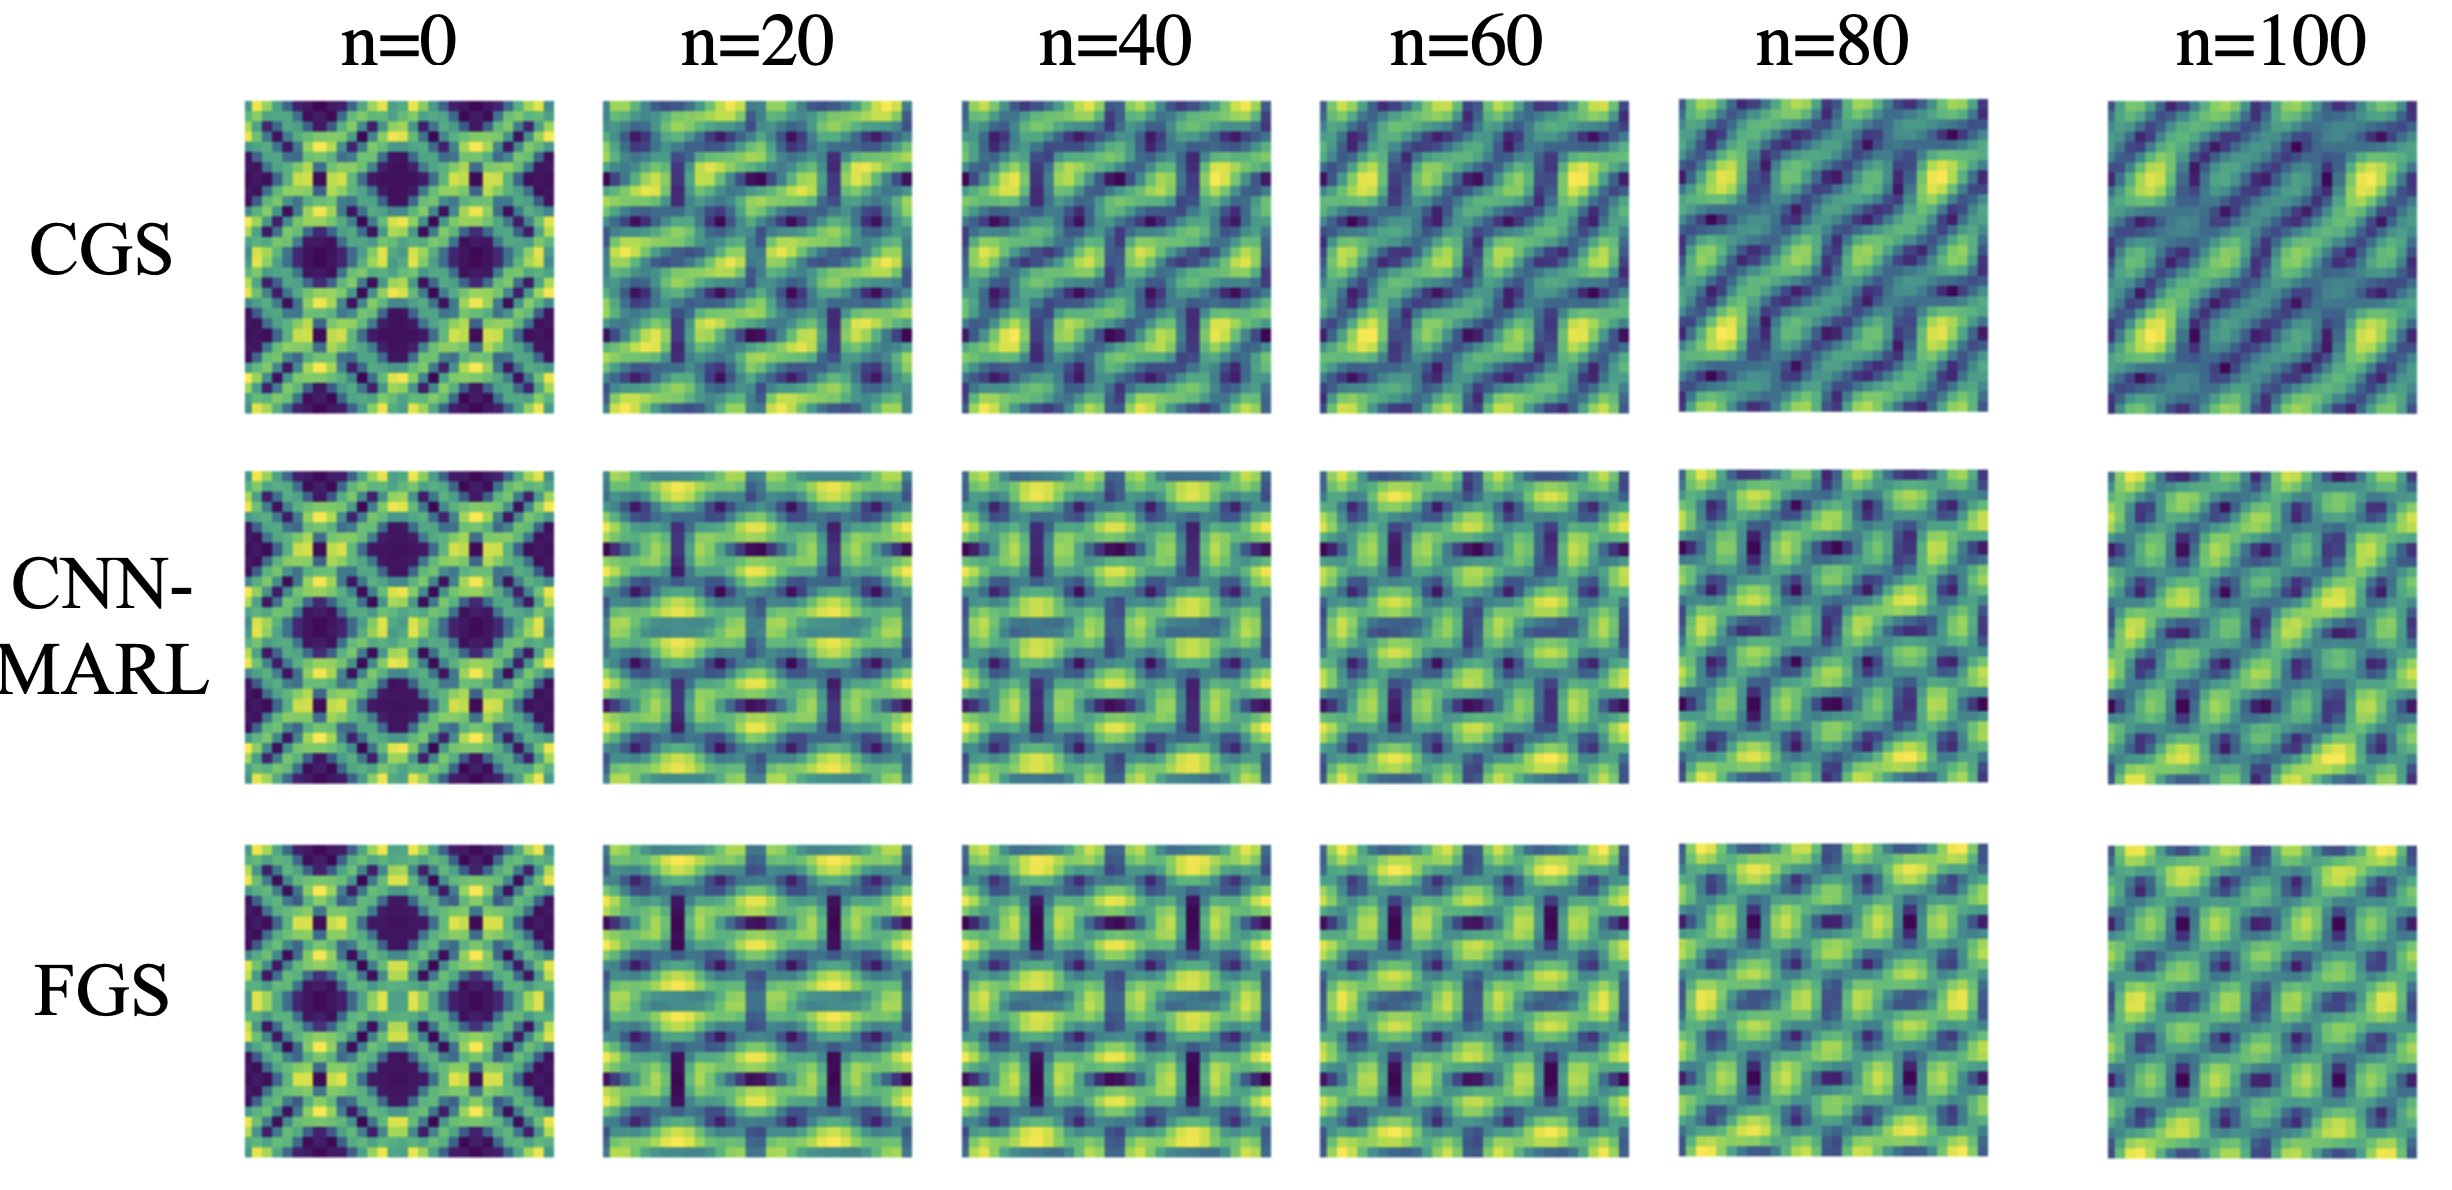
\includegraphics[width=0.75\columnwidth]{illustrations/burgers/burgers_expl1.png}}
\caption{$\boldsymbol \psi^0$ is a sample from $\mathcal D_{Train}^{Vortex}$. We plot the velocity magnitude of every $20$th step of simulation with $100$ coarse time steps. The example shows that CNN-MARL does also qualitatively keep the simulation closer to the FGS. The failure of the CGS to account for the subgrid-scale dynamics leads to diverging trajectories.}
\label{fig:burgers_example}
\end{center}
\vskip -0.2in
\end{figure}

\begin{figure}[ht]
\vskip 0.2in
\begin{center}
\centerline{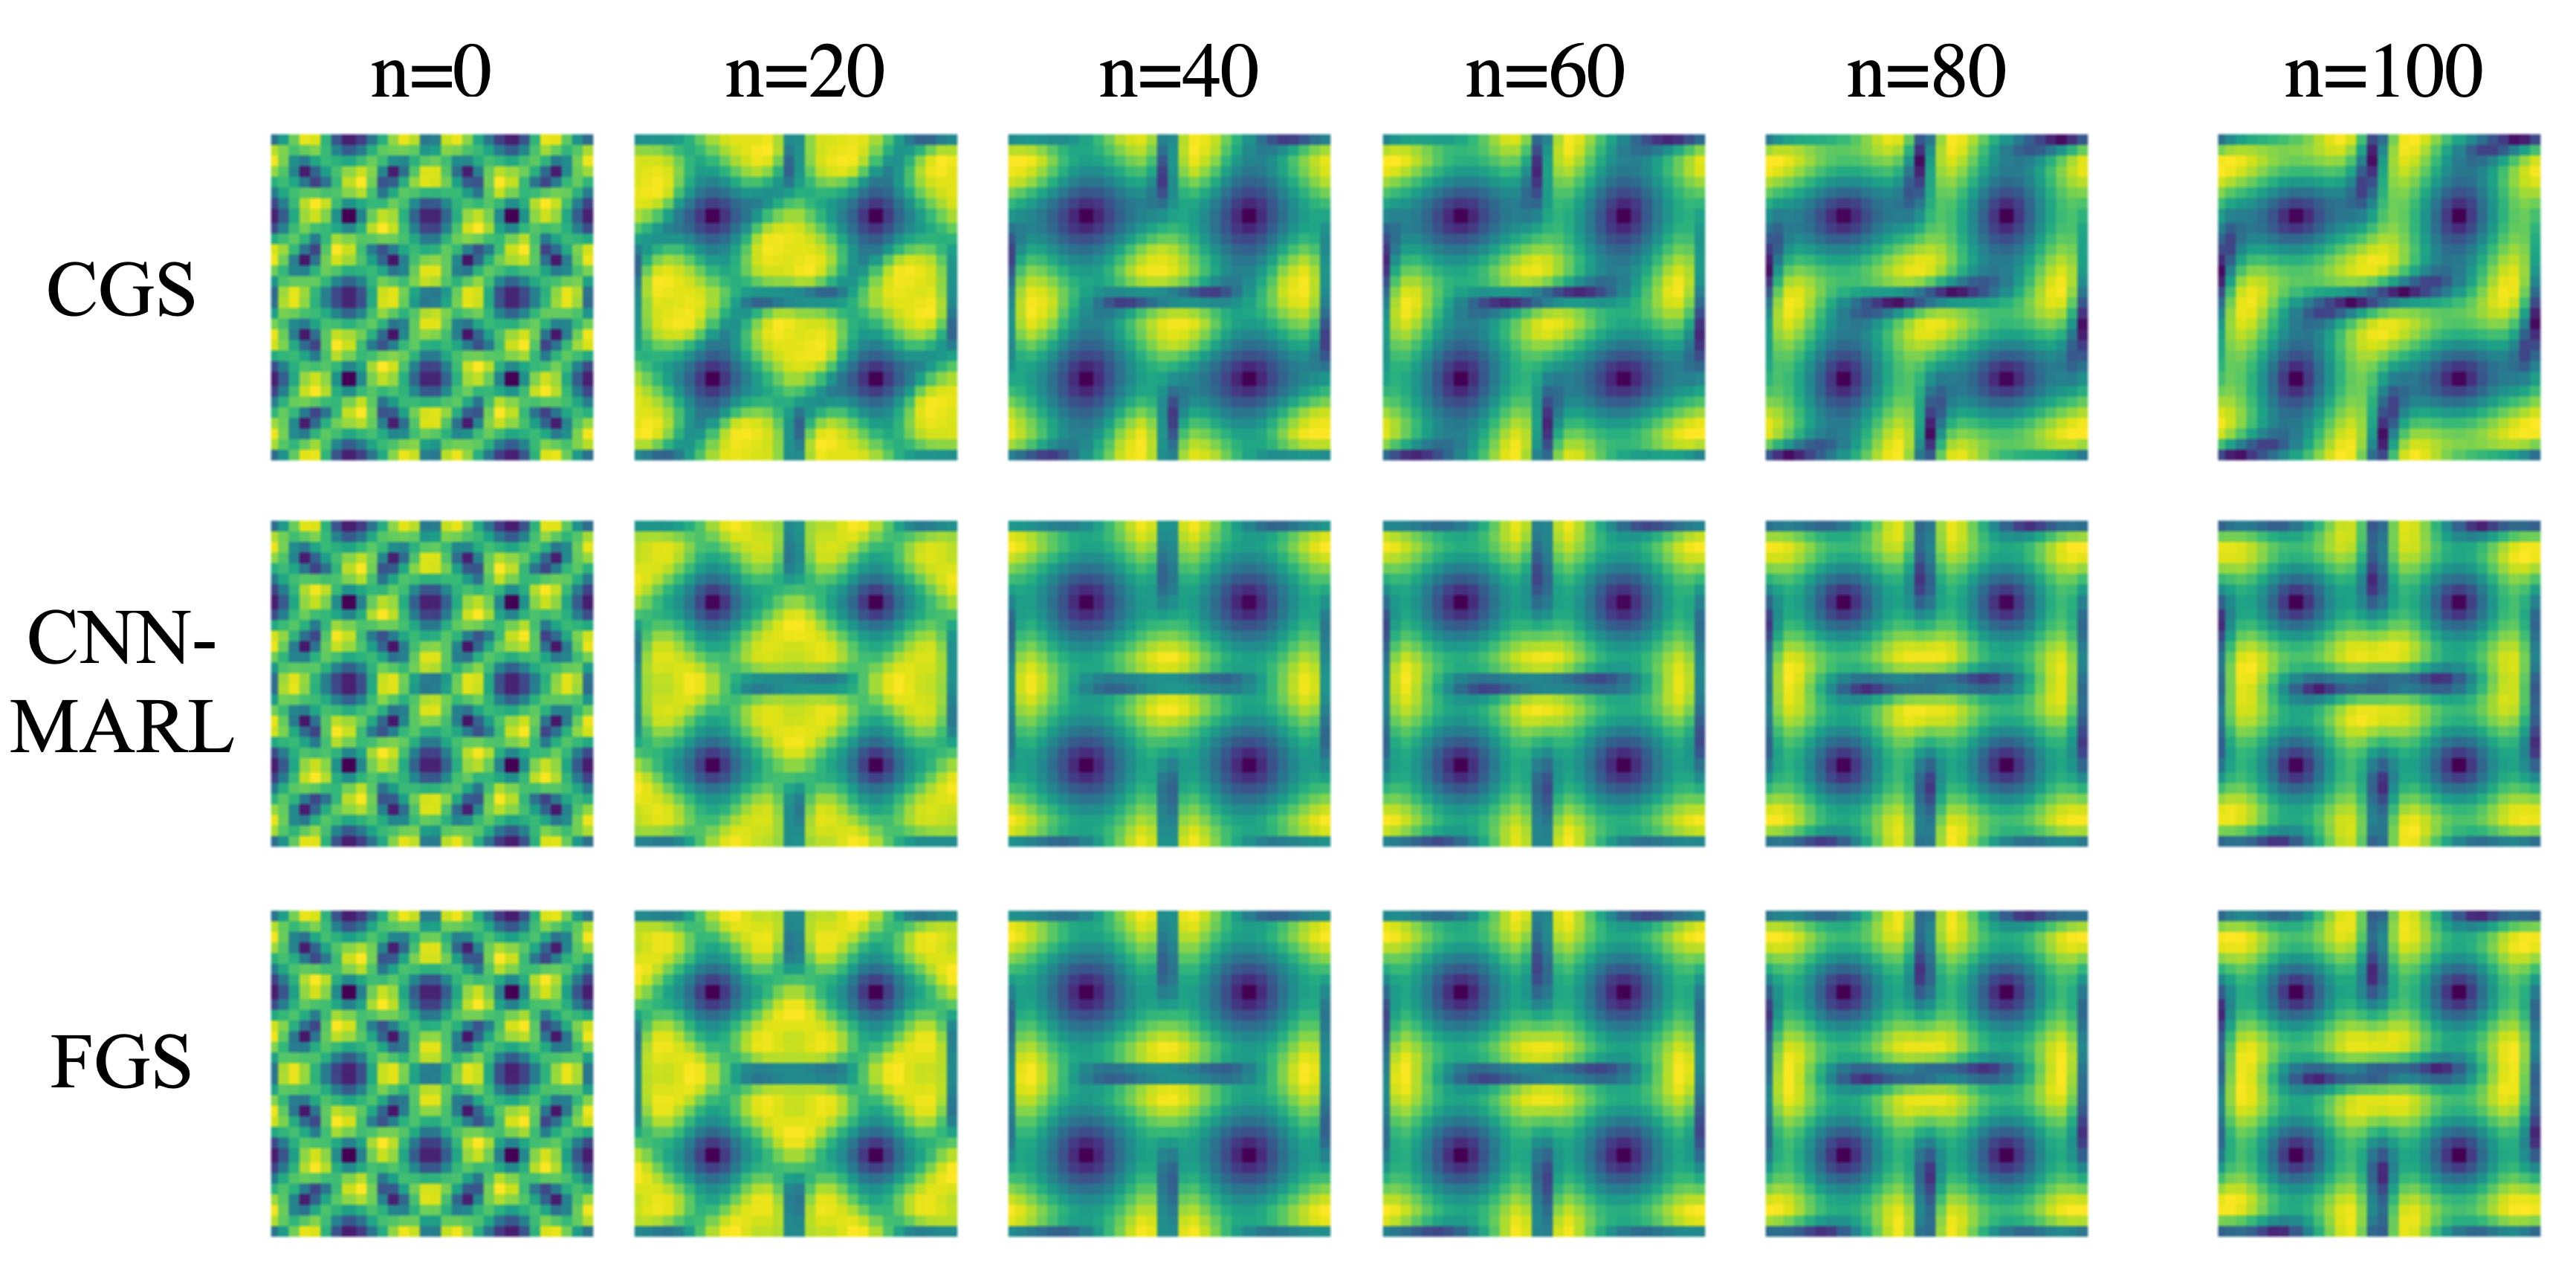
\includegraphics[width=0.75\columnwidth]{illustrations/burgers/burgers_expl2.png}}
\caption{Velocity magnitude plotted for a 100-step roll out. The set-up is the same as in \cref{fig:burgers_example} and the example again shows, that CNN-MARL leads to qualitatively different dynamics during a roll-out that are closer to those of the FGS.}
\end{center}
\vskip -0.2in
\end{figure}

\newpage
\section{Technical Details on Hyperparamters and Training Runs} \label{sec:training_hyperparams}
During training, we use entropy regularization in the PPO objective with a factor of $0.1$ and $0.05$ for the advection and Burgers' equation respectively to encourage exploration. The discount factor is set to $0.95$ and the learning rate to $1\cdot 10^{-5}$. Training is done over 2000 epochs. In each epoch, 1000 transitions are collected. One policy network update is performed after having collected one new episode. We use a batch size of 10 for training. The total number of trainable parameters amounts to $188,163$ and the entire training procedure took about 8 hours for the advection equation on an Nvidia A100 GPU. For the Burgers' equation, training took about $30$ hours on the same hardware. We save the policy every 50 epochs and log the corresponding MAE between CGS and FGS after 50 time steps. For evaluation on the advection equation, we chose the policy from epoch 1500 because it had the lowest logged MAE value. \cref{fig:advection_training_graphs} and \cref{fig:burgers_training_graphs} show the reward curves and evolutions of episode lengths. As expected, the episode length increases as the agents become better at keeping the CGS and FGS close to each other. 

\begin{figure}[h]
    \centering
    \hfill
    \raisebox{-\height}{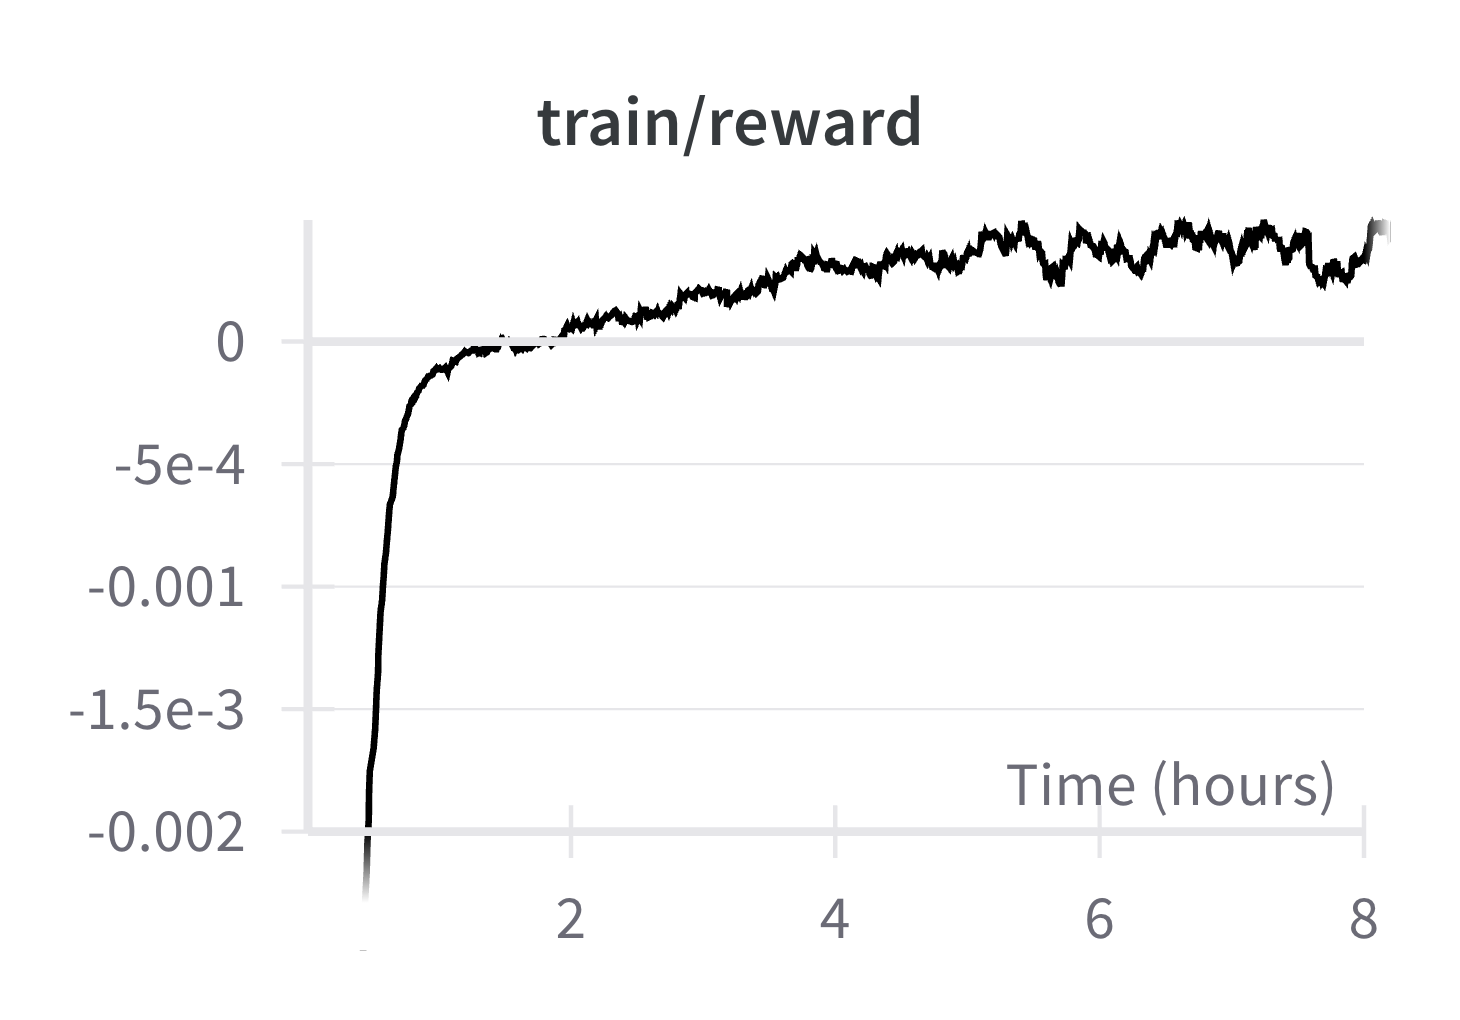
\includegraphics[width=0.4\linewidth]{figures/advection/training/train_reward.png}}
    \hfill
    \raisebox{-\height}{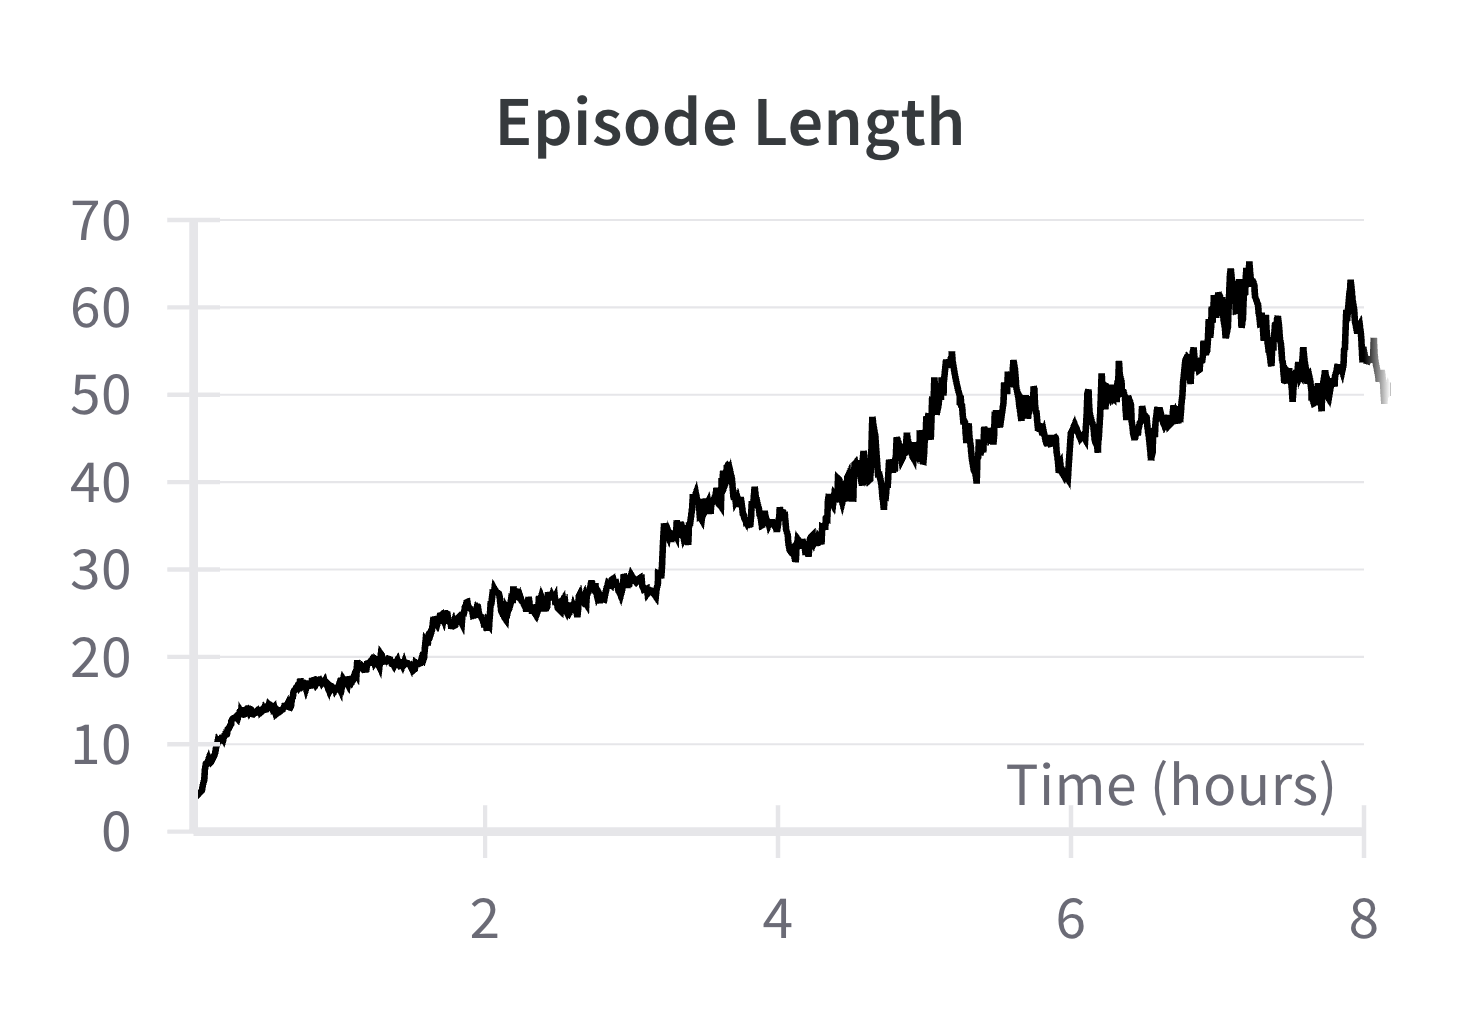
\includegraphics[width=0.4\linewidth]{figures/advection/training/train_length.png}}
    \hfill
    \caption{Visualizations of the evolution of the reward metric averaged over the agents and episode length during training on the advection equation.}
    \label{fig:advection_training_graphs}
\end{figure}

\begin{figure}[h]
    \centering
    \centering
    \hfill
    \raisebox{-\height}{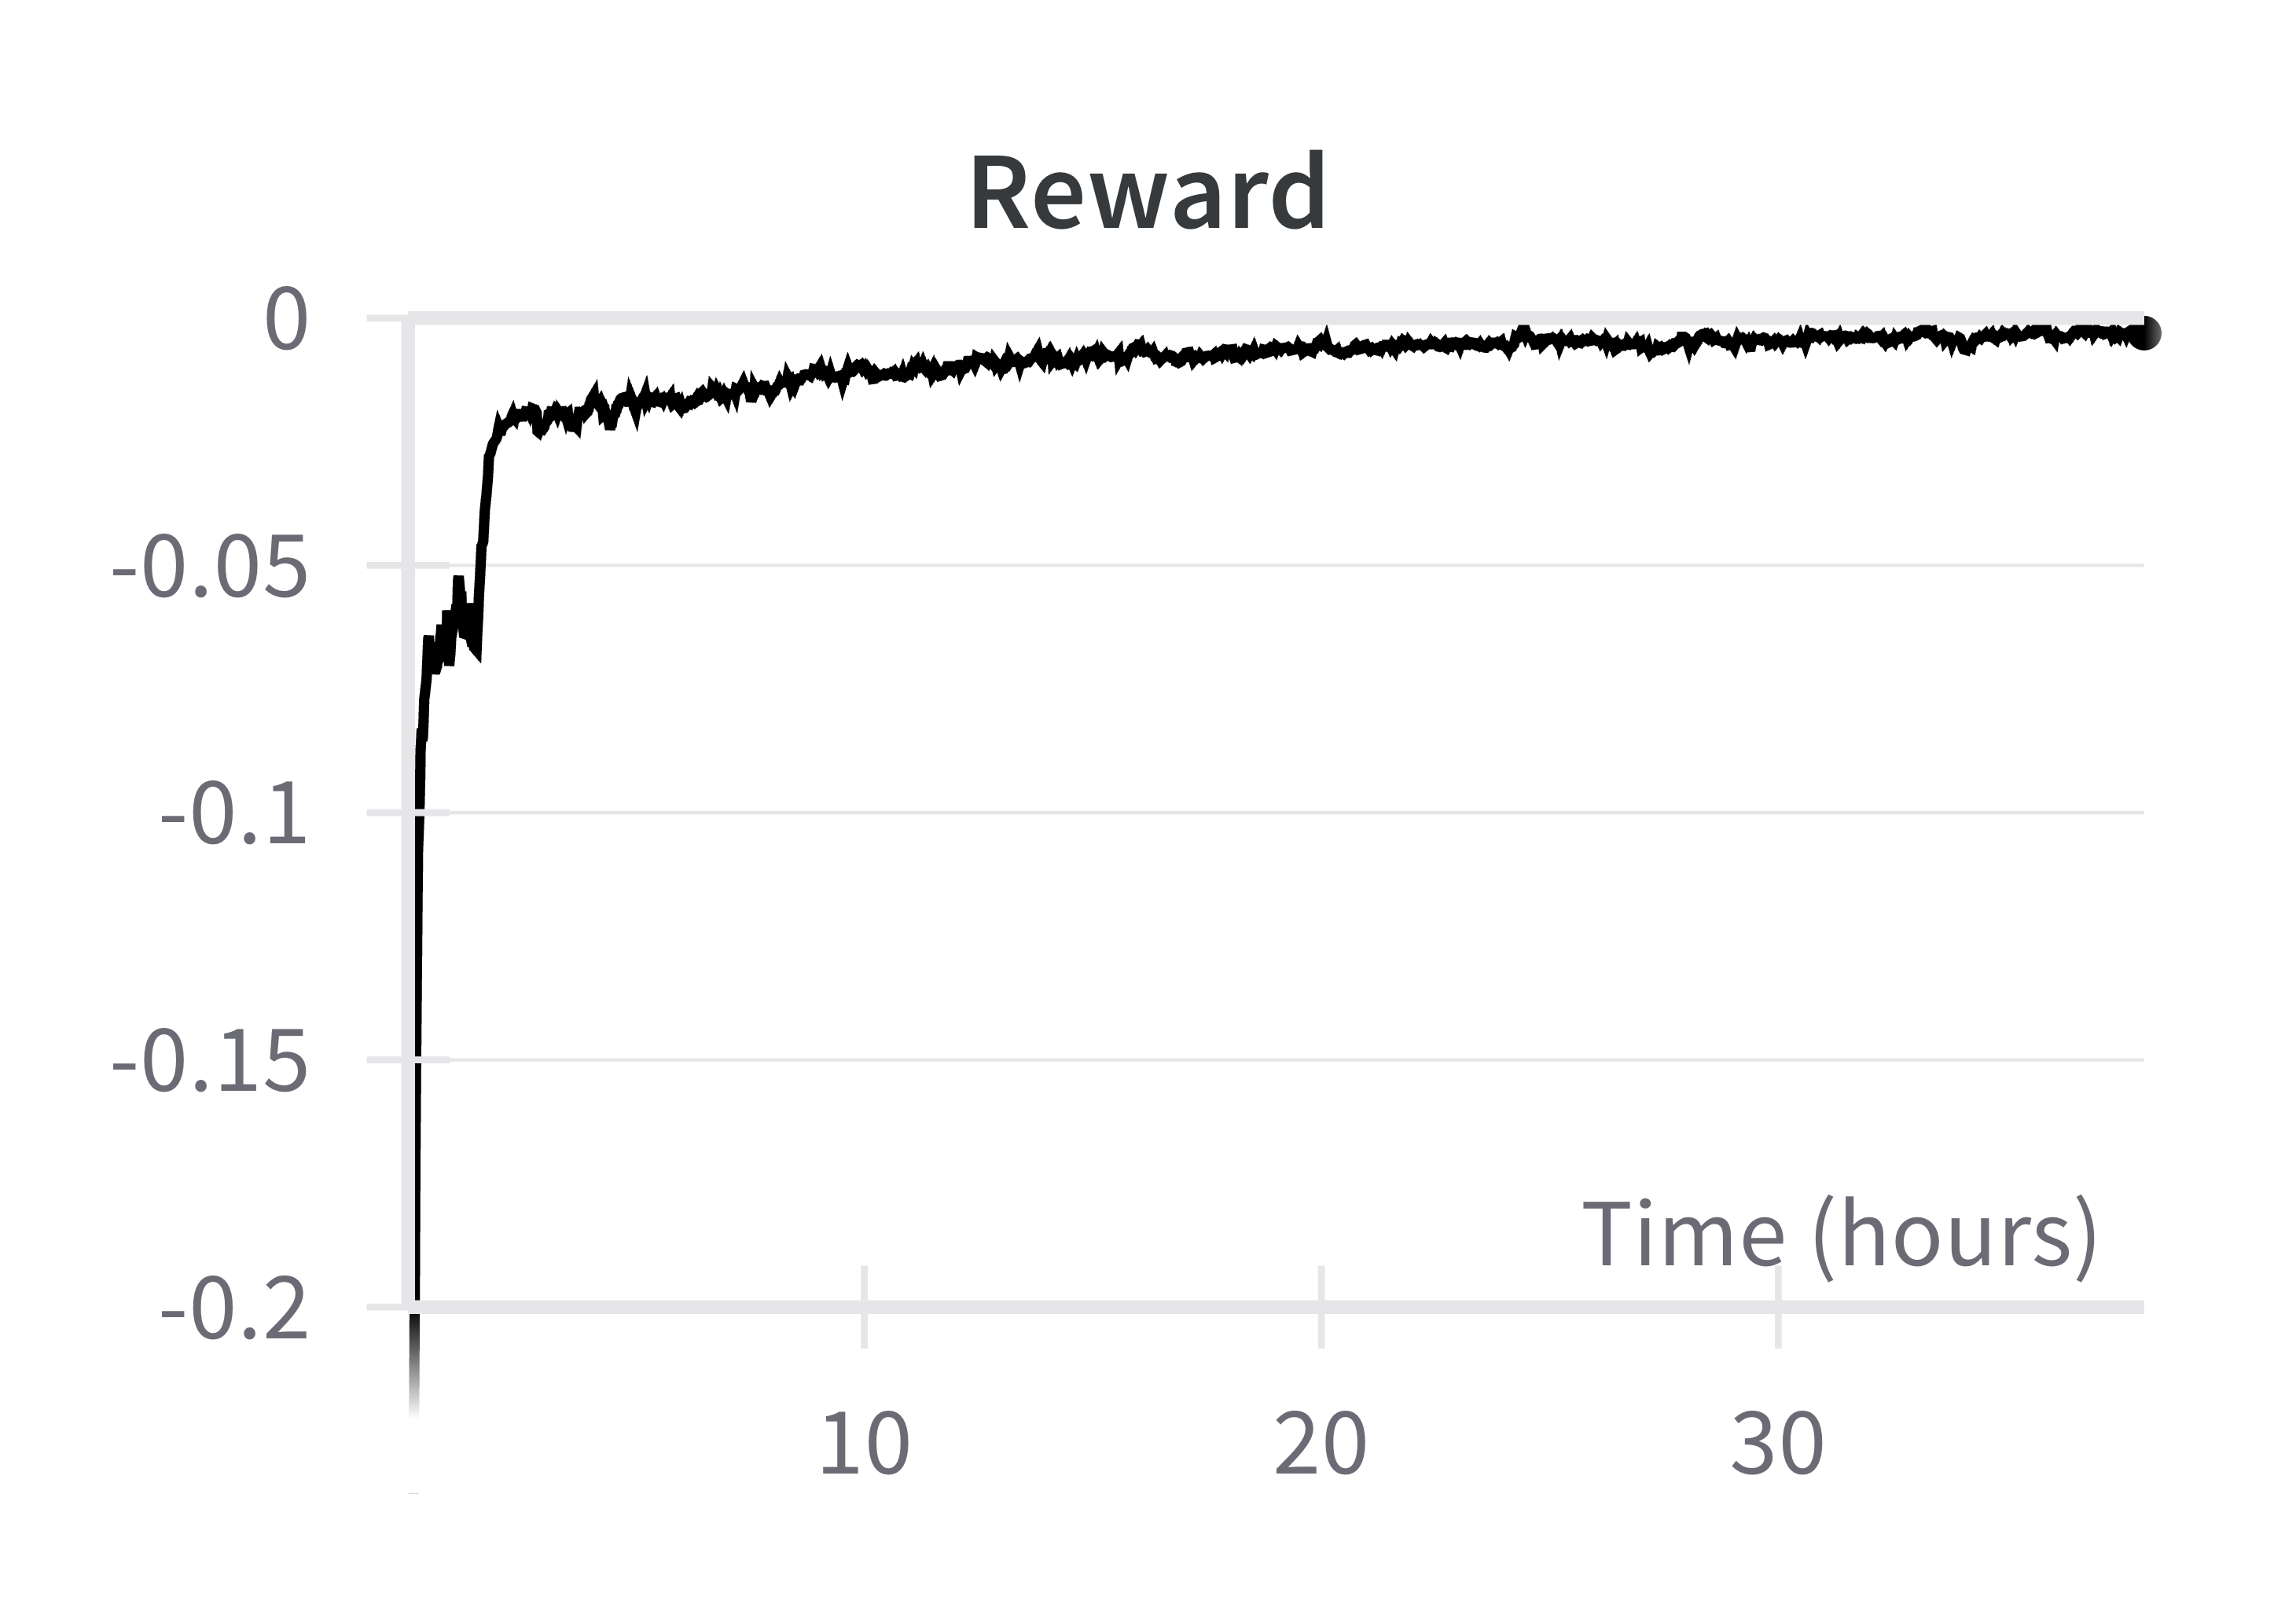
\includegraphics[width=0.4\linewidth]{figures/burgers/training/train_reward.png}}
    \hfill
    \raisebox{-\height}{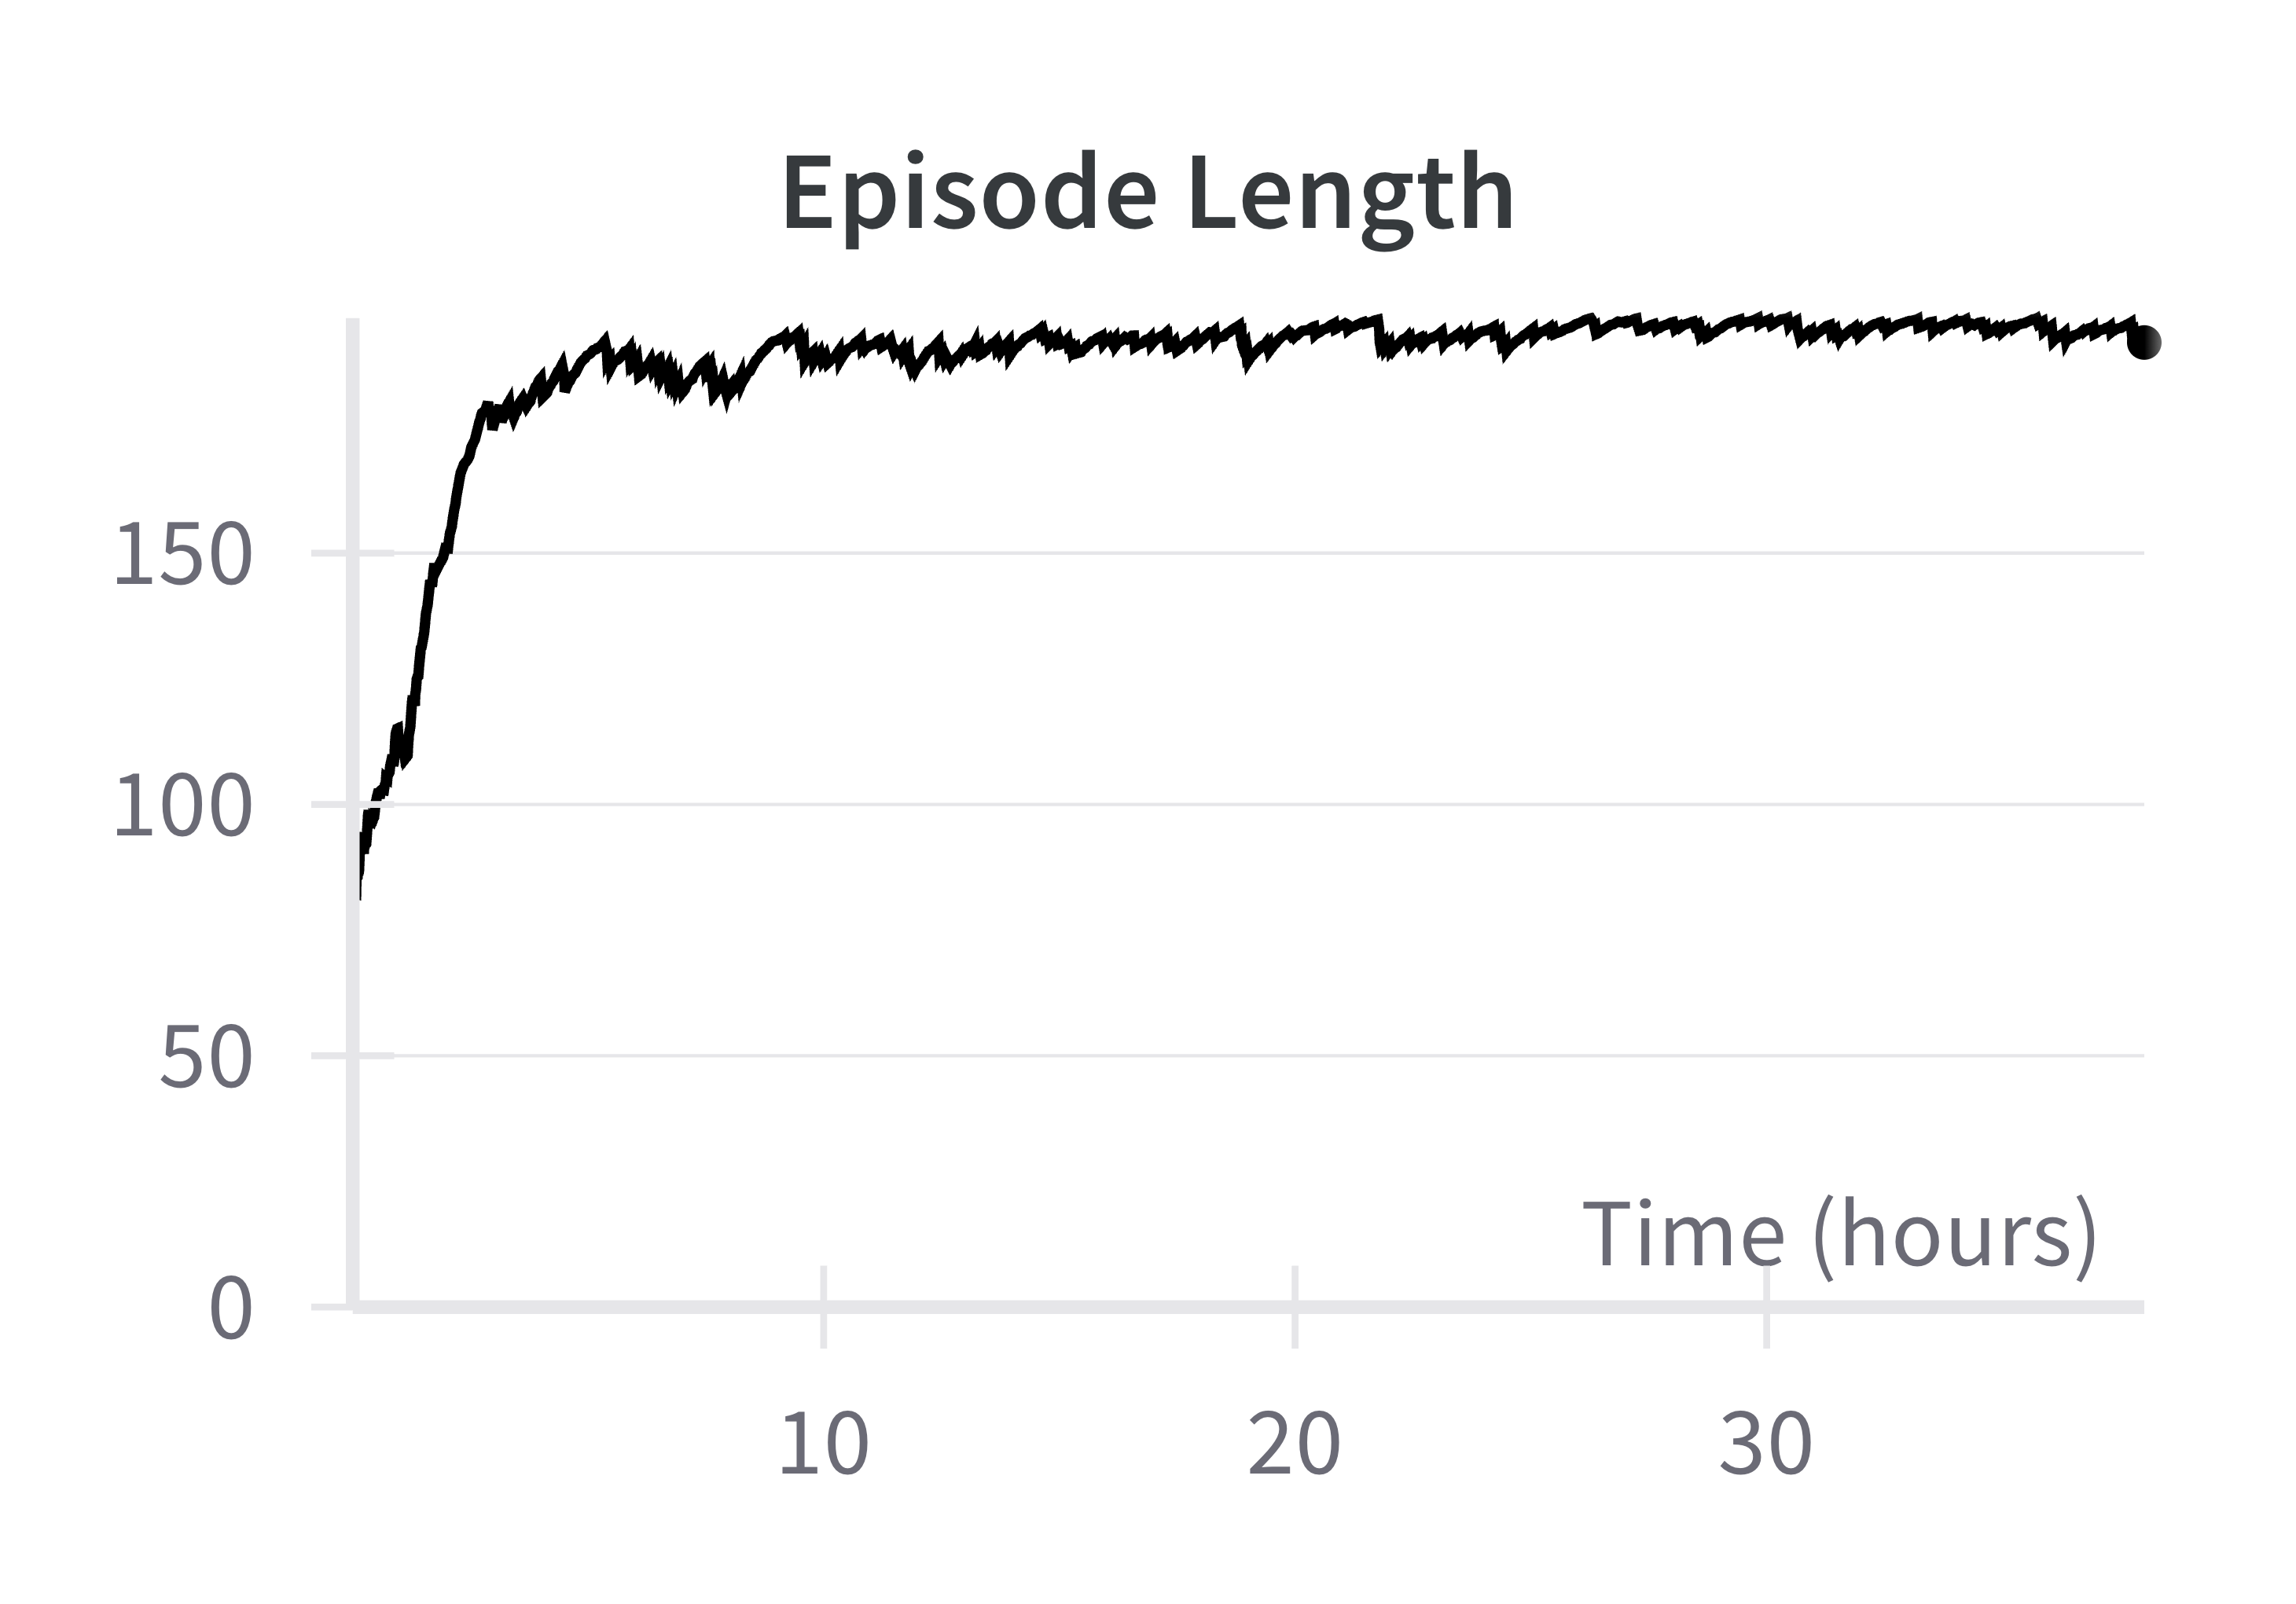
\includegraphics[width=0.4\linewidth]{figures/burgers/training/train_length.png}}
    \hfill
    \caption{Visualizations of the evolution of the reward metric averaged over the agents and episode length during training on the Burgers' equation.}
    \label{fig:burgers_training_graphs}
\end{figure}

\begin{table}[!ht]
\caption{Numerical values of the simulation parameters used for the advection CGS and FGS. Note that $\widetilde{\Delta t}$ is chosen to guarantee that the CFL condition in the CGS is fulfilled.}
\vskip 0.15in
\centering
\begin{tabular}{@{}l|c|l@{}}
\toprule
$\Omega$ & \multicolumn{2}{c}{$[0, 1] \times [0, 1]$} \\ 
$\tilde N_x$, $\tilde N_y$ & \multicolumn{2}{c}{64}  \\ 
$d, d_t$ &  \multicolumn{2}{c}{4}\\ 
\bottomrule
\multicolumn{3}{c}{Resulting other parameters:}  \\
\toprule
$ N_x$, $ N_y$ &   $d\cdot\tilde N_x,d\cdot \tilde N_y$ & $=256$ \\ 
$\Delta x, \Delta y$ &  $1/N_{x},1/N_y$ & $\approx 0,0039$  \\ 
$\widetilde{\Delta x}, \widetilde{\Delta y}$ &  $1/{\tilde N_{x}}, 1/{\tilde N_y}$ & $\approx 0,0156$   \\
$\widetilde{\Delta t}$ &  $0.9 \cdot \min(\widetilde{\Delta x}, \widetilde{\Delta y})$& $ \approx 0,0141$  \\
${\Delta t}$ &  $\widetilde{\Delta t}/{d_t}$  & $ \approx 0,0035$  \\ 
\bottomrule
\multicolumn{3}{c}{Discretization schemes:}  \\
\toprule
FGS, Space & \multicolumn{2}{c}{Central difference} \\
FGS, Time & \multicolumn{2}{c}{Fourth-order Runge-Kutta} \\
CGS, Space & \multicolumn{2}{c}{Upwind} \\
CGS, Time & \multicolumn{2}{c}{Forward Euler} \\
\bottomrule
\end{tabular}
\label{tab:advection_params}
\end{table}

\begin{table}[!ht]
\caption{Numerical values of the simulation parameters used for the Burgers' CGS and FGS. Again, $\widetilde{\Delta t}$ is chosen to guarantee that the CFL condition in the CGS is fulfilled.}
\vskip 0.15in
\centering
\begin{tabular}{@{}l|c|l@{}}
\toprule
$\Omega$ & \multicolumn{2}{c}{$[0, 1] \times [0, 1]$} \\ 
$\tilde N_x$, $\tilde N_y$ & \multicolumn{2}{c}{30}  \\ 
$d, d_t$ &  \multicolumn{2}{c}{5, 10}\\ 
\bottomrule
\multicolumn{3}{c}{Resulting other parameters:}  \\
\toprule
$ N_x$, $ N_y$ &   $d\cdot\tilde N_x,d\cdot \tilde N_y$ & $=150$ \\ 
$\Delta x, \Delta y$ &  $1/N_{x},1/N_y$ & $\approx 0,0067$  \\ 
$\widetilde{\Delta x}, \widetilde{\Delta y}$ &  $1/{\tilde N_{x}}, 1/{\tilde N_y}$ & $\approx 0,0333$   \\
$\widetilde{\Delta t}$ &  $0.9 \cdot \min(\widetilde{\Delta x}, \widetilde{\Delta y})$ & $ = 0,03$  \\
${\Delta t}$ &  $\widetilde{\Delta t}/{d_t}$ & $ = 0,003$  \\ 
\bottomrule
\multicolumn{3}{c}{Discretization schemes:}  \\
\toprule
FGS, Space & \multicolumn{2}{c}{Upwind} \\
FGS, Time & \multicolumn{2}{c}{Forward Euler} \\
CGS, Space & \multicolumn{2}{c}{Upwind} \\
CGS, Time & \multicolumn{2}{c}{Forward Euler} \\
\bottomrule
\end{tabular}
\label{tab:burgers_params}
\end{table}

\newpage
\subsection{Receptive Field of FCN}
In our CNN-MARL problem setting, the receptive field of the FCN corresponds to the observation $O_{ij}$ the agent at point $(i, j)$ is observing. In order to gain insight into this, we analyze the receptive field of our chosen architecture.

In the case of the given IRCNN architecture, the size of the receptive field (RF) of layer $i$ can be recursively calculated given the RF of layer afterward with
\begin{align}
    \text{RF}_{i+1} 
    &= \text{RF}_{i} + (\text{Kernel Size}_{i+1} - 1) \cdot \text{Dilation}_{i+1}\\
    &= \text{RF}_{i} + 2 \cdot \text{Dilation}_{i+1}.\\
\end{align}
The RF field of the first layer $\text{RF}_1$ is equal to its kernel size. By then using the recursive rule, we can calculate the RF at each layer and arrive at a value of $\text{RF}_7 = 33$ for the entire network. From this, we now arrive at the result that agent $(i,j)$ sees a $33 \times 33$ patch of the domain centered around its own location.
\begin{table}[h] 
\caption{Hyperparameters of each of the convolutional layers of the neural network architecture used for the advection equation experiment and the resulting receptive field (RF) at each layer. For the Burgers' equation experiment the architecture is simply adapted by setting the number of in channels of \texttt{Conv2D\_1} to 2 and the number of out channels of $\texttt{Conv2D}\_\pi$ to 4.} 
\vskip 0.15in
\centering
\begin{tabular}{|c|c|c|c|c|c|c|}
\hline
Layer & In Channels & Out Channels & Kernel & Padding & Dilation & RF \\
\hline
\texttt{Conv2D\_1} & 3 & 64 & 3 & 1 & 1 & 3\\
\hline
\texttt{Conv2D\_2} & 64 & 64 & 3 & 2 & 2 & 7 \\
\hline
\texttt{Conv2D\_3} & 64 & 64 & 3 & 3 & 3 & 13 \\
\hline
\texttt{Conv2D\_4} & 64 & 64 & 3 & 4 & 4 & 21 \\
\hline
\texttt{Conv2D\_5} & 64 & 64 & 3 & 3 & 3 & 27 \\
\hline
\texttt{Conv2D\_6} & 64 & 64 & 3 & 2 & 2 & 31 \\
\hline
\texttt{Conv2D}\_$\pi$ & 64 & 2 & 3 & 1 & 1 & 33 \\
\hline
\texttt{Conv2D}\_$\mathcal V$ & 64 & 1 & 3 & 1 & 1 & 33 \\
\hline
\end{tabular}
\label{tab:ircnn}
\end{table}

\subsection{Diverse Velocity Field Generation}
\subsubsection{Distribution for Training}\label{sec:train_vortices}
For the advection equation experiment, the velocity field is randomly generated by taking a linear combination of Taylor-Greene vortices and an additional random translational field. Let $\boldsymbol u_{ij}^{TG,k}, \boldsymbol v_{ij}^{TG,k}$ be the velocity components of the Taylor Greene Vortex with wave number $k$ that are defined as
\begin{align}
    \boldsymbol u_{ij}^{TG,k} &:= \cos(k\boldsymbol x_{i}) \cdot \sin(k \boldsymbol y_j) \\
    \boldsymbol v_{ij}^{TG,k} &:= - \sin(k\boldsymbol x_i) \cdot \cos(k\boldsymbol y_h).
\end{align}
Furthermore, define the velocity components of a translational velocity field as $u^{TL}, v^{TL} \in \mathbb R$. To generate a random incompressible velocity field, we sample 1 to 4 $k$'s from the set $\{1, ..., 6\}$.
For each $k$, we also sample a $\text{sign}_k$ uniformly from the set $\{-1, 1\}$ in order to randomize the vortex directions. For an additional translation term, we sample $u^{TL}, v^{TL}$ independently from  $\text{uniform}(-1, 1)$. We then initialize the velocity field to
\begin{align}
    \boldsymbol u_{ij} &:= u^{TL} + \sum_k \text{sign}_k \cdot \boldsymbol u_{ij}^{TG,k}\\
    \boldsymbol v_{ij} &:= v^{TL} + \sum_k \text{sign}_k \cdot \boldsymbol v_{ij}^{TG,k}.
\end{align}
We will refer to this distribution of vortices as $\mathcal D^{Vortex}_{Train}$. 

For the Burgers' equation experiment, we make some minor modifications to the sampling procedure. The sampling of translational velocity components is omitted and $2$ to $4$ $k$'s are sampled from $\{2, 4, 6, 8\}$. The latter ensures that the periodic boundary conditions are fulfilled during initialization which is important for the stability of the simulations.

\subsubsection{Distribution for Testing} \label{sec:test_vortices}
First, a random sign \( \text{sign} \) is sampled from the set \(\{-1, 1\}\). Subsequently, a scalar \( a\) is randomly sampled from a uniform distribution bounded between 0.5 and 1. The randomization modulates both the magnitude of the velocity components and the direction of the vortex, effectively making the field random yet structured. The functional forms of \(\boldsymbol u_{ij}^{C}\) and \(\boldsymbol v_{ij}^{C}\) are then expressed as
\begin{align}
    \boldsymbol u_{ij}^{V} &:= \text{sign} \cdot  a \cdot \sin^2(\pi \boldsymbol x_i) \sin(2\pi \boldsymbol y_j) \\
    \boldsymbol v_{ij}^{V} &:= - \text{sign} \cdot a \cdot\sin^2(\pi \boldsymbol y_j) \sin(2\pi \boldsymbol x_i).
\end{align}
In the further discussion, we will refer to this distribution of vortices as $\mathcal D^{Vortex}_{Test}$.

\subsection{Computational Complexity}
To quantitatively compare the execution times of the different simulations, we measure the runtime of performing one update step of the environment and report them in \cref{tab:execution_times}. As expected, CNN-MARL increases the runtime of the CGS. However, it stays below the FGS times by at least a factor of $5$. The difference is especially pronounced in the example of the advection equation, where the FGS uses a high order scheme on a fine grid, which leads to an execution time difference between CNN-MARL and FGS of more than an order of magnitude.
\begin{table}[t] 
\caption{Runtime of one simulation step in ms of the different simulations averaged over 500 steps.}
\label{tab:execution_times}
\vskip 0.15in
\begin{center}
\begin{scriptsize}
\begin{sc}
\begin{tabular}{l|cccr}
\toprule
 & CGS & ACGS & CNN-MARL & FGS \\
\midrule
Advection    & $\tiny 0.31 \pm 0.00$& $\tiny 0.96 \pm 0.00$& $\tiny 2.66 \pm 0.96$ & $\tiny 89.52 \pm 0.47$ \\
Burgers' & $\tiny 0.25 \pm 0.00$ & -& $\tiny 1.82 \pm 0.01$ & $\tiny 10.16 \pm 0.03$\\
\bottomrule
\end{tabular}
\end{sc}
\end{scriptsize}
\end{center}
\vskip -0.1in
\end{table}

\newpage
\section{Proof: Theoretically Optimal Action} \label{sec:proof_optimal_action}
To explore how the actions of the agents can be interpreted, we analyze the optimal actions based on the used numerical schemes. The \textit{perfect} solution would fulfill 
$$
 \mathcal{M}( \tilde{\boldsymbol \psi^n}) +\tilde{ \boldsymbol \epsilon^n}  = 0.
$$

Here, $\mathcal{M}$ is the numerical approximation of the PDE an  $\tilde{\boldsymbol \epsilon^n}$ is the truncation error.

We refer to the numerical approximations of the derivatives in the CGS as $\mathcal{T}^{FE}$ for forward Euler and $\mathcal{D}^{UW}$ for the upwind scheme. We obtain
\begin{align}
    0 &=  \mathcal{M}(\tilde{\boldsymbol\psi^n})+ \tilde{\boldsymbol\epsilon}^n\\
     &=\mathcal{T}^{FE}(\tilde{\boldsymbol\psi}^n, \tilde{\boldsymbol\psi}^{n+1}) + \tilde{\boldsymbol u}^n \mathcal{D}^{UW}_x(\tilde{\boldsymbol\psi}^n) + \tilde{\boldsymbol v}^n \mathcal{D}^{UW}_y(\tilde{\boldsymbol\psi}^n) + \tilde{\boldsymbol\epsilon}^n \\
     &=\frac{\tilde{\boldsymbol\psi}^{n+1} - \tilde{\boldsymbol\psi}^n}{\widetilde{\Delta t}} + \tilde{\boldsymbol u}^n \mathcal{D}^{UW}_x(\tilde{\boldsymbol\psi}^n) + \tilde{\boldsymbol v}^n \mathcal{D}^{UW}_y(\tilde{\boldsymbol\psi}^n) + \tilde{\boldsymbol\epsilon}^n. \\
\end{align}


By rewriting, we obtain the following time stepping rule
\begin{align}
   \tilde{\boldsymbol\psi}^{n+1} 
   &= \tilde{\boldsymbol\psi}^n - \widetilde{\Delta t} \left(\tilde{\boldsymbol u}^n \mathcal{D}^{UW}_x(\tilde{\boldsymbol\psi}^n) + \tilde{\boldsymbol v}^n \mathcal{D}^{UW}_y(\tilde{\boldsymbol\psi}^n) + \tilde{\boldsymbol\epsilon}^n\right)\\
   &= \tilde{\boldsymbol\psi}^n - \widetilde{\Delta t} \left(\tilde{\boldsymbol u}^n \mathcal{D}^{UW}_x(\tilde{\boldsymbol\psi}^n) + \tilde{\boldsymbol v}^n \mathcal{D}^{UW}_y(\tilde{\boldsymbol\psi}^n)\right) - \widetilde{\Delta t} \tilde{\boldsymbol \epsilon}^n\\
   &= \mathcal G(\tilde{\boldsymbol\psi}^n, \tilde C^n) - \widetilde{\Delta t} \tilde{\boldsymbol\epsilon}^n.
\end{align}

where $\tilde C^n:=(\tilde{\boldsymbol u}^n, \tilde{\boldsymbol v}^n)$. This update rule would theoretically find the \textit{exact} solution. It involves a coarse step followed by an additive correction after each step. We can define $ \tilde{\boldsymbol\phi}^{n+1} :=\tilde{\boldsymbol\psi}^{n+1} + \widetilde{\Delta t} \tilde{\boldsymbol\epsilon}^n$, to bring the equation into the same form as seen in the definition of the RL environment
$$ 
\tilde{\boldsymbol\phi}^{n+1} = \mathcal G(\tilde{\boldsymbol\phi}^{n} - \widetilde{\Delta t} \tilde{\boldsymbol\epsilon}^{n-1}, \tilde C^n),
$$
which illustrates that the optimal action at step $n$ would be the previous truncation error times the time increment
\begin{equation}
    \boxed{
    {\boldsymbol A^n}^* = \widetilde{\Delta t} \tilde{\boldsymbol\epsilon}^{n-1}.
    }
\end{equation}
